
In this section, we give the first quantum algorithm for the subset-sum problem, \emph{in the QRACM model}, with an asymptotic complexity smaller than BCJ.

\subsection{Quantum Match-and-Filter}

We open this section with some technical lemmas that replace the classical merge-and-filter Lemma~\ref{lemma:classical-merging}. In this section, we will consider a merging tree as in the HGJ algorithm, but this tree will be built using quantum search. The following lemmas bound the expected time of merge-and-filter \emph{and} match-and-filter operations performed quantumly, in the QRACM model. This will have consequences both in this section and in the next one.


%We are now going to remark that Grover search, in the QRACM model, improves the merging with filtering operation, \emph{even if the input lists are both classical}. This will have consequences both on the asymmetric HGJ and the algorithms based on quantum walks.

First, we remark that we can use a much more simple data structure than the ones in~\cite{DBLP:journals/siamcomp/Ambainis07,DBLP:conf/pqcrypto/BernsteinJLM13}. In this data structure, we store pairs $\vec{e}, \vec{e} \cdot \vec{a}$ indexed by $\vec{e} \cdot \vec{a} \mod M$ for some $M \simeq 2^m$. %Since $M$ is an integer, the vectors are simply indexed by $i \leq M$.% In addition, we can store $B$ vectors for a given modulus instead of only 1, in which case we assume that these vectors are sorted. But in this section we need only 1 per modulus.

\begin{definition}[Unique modulus list]\label{def:unique-mod}
A \emph{unique modulus list} is a qRAM data structure $\mathcal{L}(M)$ that stores at most $M$ entries $(\vec{e}, \vec{e} \cdot \vec{a})$, indexed by $\vec{e} \cdot \vec{a} \mod M$, and supports the following operations:
\begin{itemize}
\item Insertion: inserts the entry $(\vec{e}, \vec{e} \cdot \vec{a})$ if the modulus is not already occupied;
\item Deletion: deletes $(\vec{e}, \vec{e} \cdot \vec{a})$ (not necessary in this section)
\item Query in superposition: returns the superposition of all entries $(\vec{e}, \vec{e} \cdot \vec{a})$ with some modular condition on $\vec{e} \cdot \vec{a}$, \emph{e.g.} $\vec{e} \cdot \vec{a} = t \mod M'$ for some $t$ and some modulus $M'$.
\end{itemize}
\end{definition}

Note that all of these operations, \emph{including} the query in superposition of all the entries with a given modulus, cost $\bigO{1}$ qRAM gates only. For the latter, we need only some Hadamard gates to prepare the adequate superposition of indices. Furthermore, the list remains sorted by design.

%The \emph{unique modulus list} is actually the quantum analogous of a classical RAM data structure.


%First, we remark that by using an adapted data structure as in~\cite{DBLP:conf/pqcrypto/BernsteinJLM13}, we can use the QRACM model for finding \emph{partial matching elements}, which is more general than a simple lookup. When there are multiple solutions, we obtain their uniform superposition.

%we remark that the QRACM model allows not only fast lookup of elements (using a data structure as in), but also returning the uniform superposition of partial matches, if there are many solutions.

%\XB{Il m'a l'air un peu bizarre, ce lemme. Pour moi, on y arrive de la même façon qu'en classique : avec des listes triées. Sinon, je ne vois pas ce qui ferait que ça marche différemment du matching, en fait. (Donc dans le détail ça donnerait: par dichotomie, on obtient l'intervalle des solutions, on produit la superposition des indices correspondant en temps poly, on fait la requête. J'ai manqué un truc ?)}
%\begin{lemma}[QRACM query with multiple answers]\label{lemma:QRACM-multiple}
%Let $M$ be a memory of size $2^m$ holding $n$-bit strings $x_0, \ldots x_{2^m-1}$. Then in the QRACM model, there exists a data structure for $M$ that
%%Let $M$ be a QRACM memory of size $2^m$ holding $n$-bit strings $x_0, \ldots x_{2^m-1}$. Then it 
%can answer, in $\poly(m,n)$ time, partial matching queries with multiple answers:
%$$ \ket{y} \ket{0}, s \mapsto \ket{y} \sum_{ i | y \oplus x_i \text{ starts with } s } \ket{i} \enspace.$$
%%by returning a uniform superposition over the QRACM indices of the elements that satisfy the partial collision condition.
%\end{lemma}

%\begin{proof}[Sketch]
%In the case where there are many solutions, divide the QRACM into arbitrary chunks such that each chunk has on average one solution. Then, perform a query for each chunk, in superposition over the chunk indices. \qed
%\end{proof}

%\begin{lemma}[Quantum merging with filtering]\label{lemma:quantum-merging-filtering}
%Let $L_1$ and $L_2$ be two lists stored in QRACM. Then assuming that it contains at least one element, the filtered joint list $L_1 \bowtie_c L_2$, with a $nc$-bit modular condition, and a filtering term $f$, can be written in time: 
%$$  \frac{1}{\sqrt{f}} \max \left(\min \left( |L_1| \sqrt{\frac{|L_2|}{2^c}} , |L_2| \sqrt{\frac{|L_1|}{2^c}} \right)  , \frac{|L_1| |L_2|}{2^c} \right) \enspace.$$. 
%\end{lemma}
%
%\begin{proof}
%Assume as before that we start from list $L_1$. Let us consider separately three cases:
%\begin{itemize}
%\item $|L_2| < 2^c$: there is on average less than one element to get from $L_2$, and we must loop over $2^c / |L_2|$ elements of $L_1$ before we find one. Since we must also filter a proportion $1/f$ of the partial solutions, we use a Grover search over $2^c f / |L_2|$ elements of $L_1$, to find a single expected solution. We repeat this before we get all elements in the final (filtered) list, hence $ |L_1| |L_2| / (2^c f) $ times, for a total time complexity:
%$$ \sqrt{ \frac{2^c f}{|L_2|} } \frac{|L_1| |L_2|}{2^c f} = |L_1| \sqrt{ \frac{|L_2|}{2^c f} } \enspace. $$
%\item $|L_2| > 2^c$ and $|L_2| > 2^c f$: an element of $L_1$ yields on average more than one matching candidates in $L_2$, before and after filtering. In the classical setting, all these candidates can be produced in average time $1$ and filtered immediately. In the quantum setting, the superposition of all candidates can be produced in time $1$, by a QRACM query with multiple answers (Lemma~\ref{lemma:QRACM-multiple}). Classically, after filtering a chunk of $f$ candidates, we expect one solution; here we perform a Grover search on such a chunk. Instead of having $f$ classical steps, it will have $\sqrt{f}$ iterations. The total time is:
%$\frac{|L_1| |L_2|}{2^c f} \times \sqrt{f} = \frac{|L_1| |L_2|}{2^c \sqrt{f}} \enspace.$
%\item $|L_2| > 2^c$ and $|L_2| < 2^c f$: an element of $L_1$ yields on average more than one matching candidates in $L_2$ before filtering, but less than one after filtering. The situation is the same as before. The only change is that our ``chunks of candidates'' actually contain pairs of vectors $e_1, e_2$ with varying $_e2$ \emph{and} $e_1$. But the superposition over a chunk can still be produced in unitary time and this does not impact the complexity. \AS{ok, maybe make this clearer}
%\end{itemize}
%
%The total time in all cases becomes (assuming that the output list contains at least one element):
%$$  \frac{1}{\sqrt{f}} \max \left(\min \left( |L_1| \sqrt{\frac{|L_2|}{2^c}} , |L_2| \sqrt{\frac{|L_1|}{2^c}} \right)  , \frac{|L_1| |L_2|}{2^c} \right) \enspace.$$
%
%Notice that it can even become smaller than $|L_1|$ and $|L_2|$, thanks to the QRACM queries (however we assumed that both the input lists were stored in QRACM, so they will have to be produced at some point). \qed
%\end{proof}

Next, we write a lemma for quantum \emph{matching} with filtering, in which one of the lists is not written down. We start from a unitary that produces the uniform superposition of the elements of a list $L_1$, and we wrap it into an amplitude amplification, in order to obtain a unitary that produces the uniform superposition of the elements of the merged-and-filtered list.


\begin{lemma}[Quantum matching with filtering]\label{lemma:quantum-matching-filtering}
Let $L_2$ be a list stored in QRACM (with the \emph{unique modulus list} data structure of Definition~\ref{def:unique-mod}). Assume given a unitary $U$ that produces in time $t_{L_1}$ the uniform superposition of $L_1 = x_0, \ldots x_{2^m -1}$ where $x_i = (\vec{e_i}, \vec{e_i} \cdot \vec{a})$.
%$$ \ket{0} \ket{0} \mapsto \sum_i \ket{i} \ket{x_i} \enspace. $$
We merge $L_1$ and $L_2$ with a modular condition of $cn$ bits and a filtering probability $p$. Let $L$ be the merged list and $L^f$ the filtered list. Assume $|L^f| \geq 1$. Then there exists a unitary $U'$ producing the uniform superposition of $L^f$ in time: $\bigO{ \frac{t_{L_1}}{\sqrt{p}} \max( \sqrt{2^{cn} / |L_2|} , 1 ) }$.
\end{lemma}

Notice that this is also the time complexity to produce a single random element of $L^f$. If we want to produce and store the whole list $L^f$, it suffices to multiply this complexity by the number of elements in $L^f$ (\emph{i.e.} $p|L_1||L_2|/2^{cn}$). We would obtain: $\bigO{ t_{L_1} \sqrt{p} \max \left( |L_1| \sqrt{\frac{|L_2|}{2^{cn}}}  , \frac{|L_1| |L_2|}{2^{cn}} \right) } \enspace.$

\begin{proof}
Since $L_2$ is stored in a unique modulus list, all its elements have distinct moduli. Note that the \emph{expected} sizes of $L$ and $L^f$ follow from Heuristic~\ref{heur1}. Although the number of iterations of quantum search should depend on the \emph{real} sizes of these lists, the concentration around the average is so high (given by Chernoff bounds) that the error remains negligible if we run the search with the expected number of iterations. We separate three cases.
\begin{itemize}
\item If $|L_2| < 2^{cn}$, then we have no choice but to make a quantum search on elements of $L_1$ that match the modular constraint and pass the filtering step, in time: $\bigO{ t_{L_1} \sqrt{ \frac{2^{cn}}{L_2 p} } }$.

\item If $|L_2| > 2^{cn}$ but $|L_2| < 2^{cn} / p$, an element of $L_1$ will always pass the modular constraint, with more than one candidate, but in general all these candidates will be filtered out. Given an element of $L_1$, producing the superposition of these candidates is done in time $1$, so finding the one that passes the filter, if there is one, takes time $\sqrt{|L_2|/2^{cn}}$. Next, we wrap this in a quantum search to find the ``good'' elements of $L_1$ (passing the two conditions), with $ \bigO{\sqrt{ 2^{cn} / p L_2}}$ iterations. The total time is:
$$\bigO{ \sqrt{ \frac{2^{cn}}{L_2 p} } \times \left(  \sqrt{|L_2|/2^{cn}} \times t_{L_1} \right) =  \frac{t_{L_1}}{\sqrt{p}} }\enspace. $$

\item If $|L_2| > 2^{cn}/ p$, an element of $L_1$ yields on average more than one filtered candidate. Producing the superposition of the modular candidates is done in time $\bigO{1}$ thanks to the data structure, then finding the superposition of filtered candidates requires $1/\sqrt{p}$ iterations. The total time is: $\bigO{ t_{L_1} / \sqrt{p} }$.
\end{itemize}
The total time in all cases is: $\bigO{ \frac{t_{L_1}}{\sqrt{p}} \max( \sqrt{2^{cn} / |L_2|} , 1 ) }$. Note that classically, the coupon collector problem would have added a polynomial factor, but this is not the case here thanks to QRACM (Remark~\ref{remark:coupon-coll}). \qed
\end{proof}



%If the filtered list contains on expectation less than one element, ie $|L_1| |L_2| < 2^c f$, then there are two situations:
%\begin{enumerate}
%\item The unfiltered list $L_1 \bowtie_c L_2$ is of expected size $< 1$, i.e. $|L_1| |L_2| < 2^c$. In that case we perform Grover search over the elements of $L_1$, looking for the expected single solution (if there is one). The time is $t_{L_1} \sqrt{|L_1|}$. Testing the filter condition is immediate.
%\item $|L_1| |L_2| > 2^c$ but after filtering, less than one element remains. Then we do two Grover searches, first for the matching pairs, then for the expected single filtered pair. The time remains $t_{L_1} \sqrt{|L_1|}$.
%\end{enumerate}

In the QRACM model, we have the following corollary for merging and filtering two lists of equal size. This result will be helpful in Section~\ref{subsection:hgj-quantum-second} and~\ref{section:new-qw}.

\begin{corollary}\label{lemma:symmetric-merging}
Consider two lists $L_1, L_2$ of size $|L_1| = |L_2| = |L|$ exponential in $n$. We merge $L_1$ and $L_2$ with a modular condition of $cn$ bits, and filter with a probability $p$. Assume that $2^{cn} < |L|$. Then $L^f$ can be written down in quantum time: $\bigO{ \sqrt{p} \frac{|L|^2}{2^{cn}} } $.
% $\bigOt{|L^f| \sqrt{ \frac{|L|^2}{2^{cn} |L^f|} } }$.%, up to a polynomial factor in $n$.
\end{corollary}

\begin{proof}
We do a quantum search to find each element of $L^f$. We have $t_{L_1} = \bigO{1}$ since it is a mere QRACM query, and we use Lemma~\ref{lemma:quantum-matching-filtering}. \qed
%Finding an element of $L^f$ costs time $\bigOt{ \sqrt{ \frac{|L|^2}{2^{cn} |L^f|} } }$. We then find all elements of $L^f$ by repeating this search (this is a coupon collector problem). \qed
% Finding all elements of $L^f$ is a coupon collector problem, and we succeed with a probability exponentially close to $1$ after $\bigO{|L^| \log |L''|}$ trials. Since $|L''|$ is only exponential in $n$, $\log |L''|$ is polynomial. \qed
\end{proof}



\subsection{Revisiting HGJ}
\label{subsection:hgj-quantum-first}

We now introduce our new algorithm for subset-sum in the QRACM model.

Our starting point is the HGJ algorithm. Similarly to~\cite{DBLP:journals/iacr/Naya-PlasenciaS19}, we use a merging tree in which the lists at a given level may have different sizes. Classically, this does not improve the time complexity. However, quantumly, we will use quantum filtering. Since our algorithm does not require to write data in superposition, only to read from classical registers with quantum random access, we require only QRACM instead of QRAQM.


In the following, we consider that all lists, except $L_0^3, L_0^2, L_0^1, L^0$, are built with classical merges. The final list $L^0$, containing (expectedly) a single element, and a branch leading to it, are part of a nested quantum search. Each list $L_0^3, L_0^2, L_0^1, L^0$ corresponds either to a search space, the solutions of a search, or both. We represent this situation on Fig.~\ref{fig:hgj-quantum}. Our procedure runs as follows:
\begin{enumerate}
\item (Classical step): build the \emph{intermediate lists} $L_1^3, L_1^2, L_1^1$ and store them using a \emph{unique modulus list} data structure (Definition~\ref{def:unique-mod}).
\item (Quantum step): do a quantum search on $L_0^3$. To test a vector $\vec{e} \in L_0^3$:
\begin{itemize}
\item Find $\vec{e}_3 \in L_1^3$ such that $\vec{e} + \vec{e}_3$ passes the $c^2_0n$-bit modular constraint (assume that there is at most one such solution). There is no filtering here.
\item Find $\vec{e}_2 \in L_1^2$ such that $(\vec{e} + \vec{e}_3) + \vec{e}_2$ passes the additional $(c^1-c^2_0)n$-bit constraint.
\item If it also passes the filtering step, find $\vec{e}_1 \in L_1^1$ such that $(\vec{e} + \vec{e}_3 + \vec{e}_2) + \vec{e}_1$ is a solution to the knapsack problem (and passes the filter).
\end{itemize}
\end{enumerate}

Structural constraints are imposed on the tree, in order to guarantee that there exists a knapsack solution. The only difference between the quantum and classical settings is in the optimization goal: the final time complexity.


\begin{figure}[htb]
\centering
\scalebox{0.8}{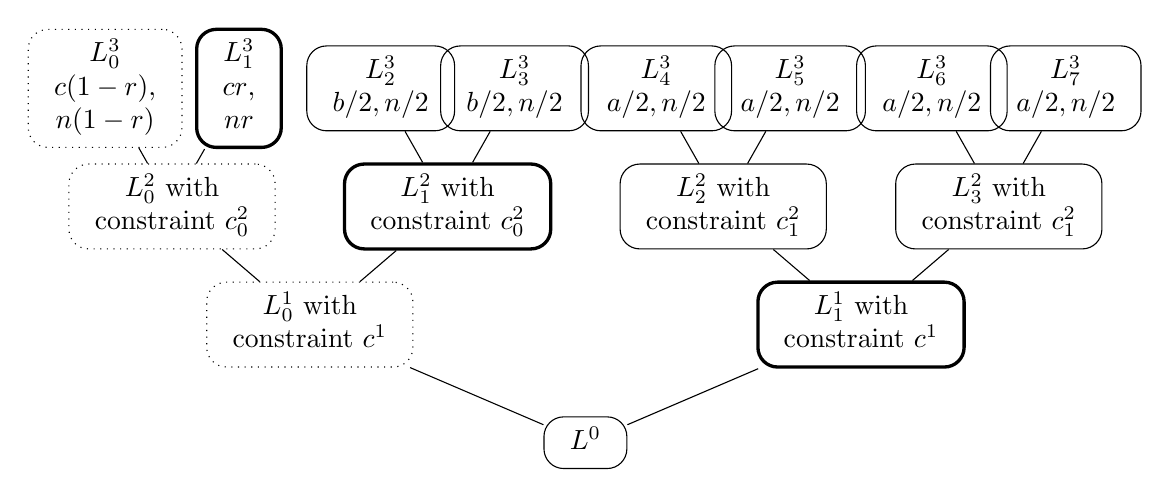
\begin{tikzpicture}[grow=up,nodes={draw,rectangle,rounded corners=.25cm,->}, level 1/.style={sibling distance=70mm}, level 2/.style={sibling distance=35mm}, level 3/.style={sibling distance=17mm}]
\node{ \begin{tabular}{c} $L^0$ \end{tabular}}
    child { node[very thick] {\begin{tabular}{c} $L_1^1$ with \\ constraint $c^1$ \end{tabular} }
    	child { node {\begin{tabular}{c} $L_3^2 $ with \\ constraint $c_1^2$ \end{tabular} }
    		child { node {\begin{tabular}{c} $L_7^3 $ \\ $a/2, n/2$\end{tabular} }}
			child { node {\begin{tabular}{c} $L_6^3 $ \\ $a/2, n/2$\end{tabular} }}}
    	child { node {\begin{tabular}{c} $L_2^2 $ with \\ constraint $c_1^2$ \end{tabular} }
			child { node {\begin{tabular}{c} $L_5^3 $ \\ $a/2, n/2$\end{tabular} }}
			child { node {\begin{tabular}{c} $L_4^3 $ \\ $a/2, n/2$\end{tabular} }} }}
    child { node[dotted] {\begin{tabular}{c} $L_0^1$ with \\ constraint $c^1$ \end{tabular} }
    	child { node[very thick] {\begin{tabular}{c} $L_1^2 $ with \\ constraint $c_0^2$ \end{tabular} }
    		child { node {\begin{tabular}{c} $L_3^3 $\\ $b/2, n/2$\end{tabular} }}
			child { node {\begin{tabular}{c} $L_2^3 $\\ $b/2, n/2$ \end{tabular} }} 
			 }
    	child { node[dotted] {\begin{tabular}{c} $L_0^2 $ with \\ constraint $c_0^2$ \end{tabular} }
			child { node[very thick]         {\begin{tabular}{c} $L_1^3 $\\ $cr$, \\ $n r$ \end{tabular} }}			
			child { node[dotted] {\begin{tabular}{c} $L_0^3 $\\ $c(1-r)$, \\ $n(1-r)$ \end{tabular} }} 
			 }};
\end{tikzpicture}}
\caption{Quantum HGJ algorithm. Dotted lists are search spaces (they are not stored). Bold lists are stored in QRACM. In Section~\ref{subsection:hgj-quantum-second}, $L_2^2$ and $L_3^2$ are also stored in QRACM.}
\label{fig:hgj-quantum}
\end{figure}

\paragraph{Structural Constraints.}
We now introduce the variables and the structural constraints that determine the shape of the tree in Fig.~\ref{fig:hgj-quantum}. The asymmetry happens both in the weights at level 0 and at the constraints at level 1 and 2. We write $\ell_i^j = (\log_2 | L_i^j|) / n$. With the lists built classically, we expect a symmetry to be respected, so we have: $\ell_2^3 = \ell_3^3$, $\ell_4^3 = \ell_5^3 = \ell_6^3 = \ell_7^3$, $\ell_2^2 = \ell_3^2$. We also tweak the left-right split at level 0: lists from $L_2^3$ to $L_7^3$ have a standard balanced left-right split; however, we introduce a parameter $r$ that determines the proportion of positions set to zero in list $L_0^3$: in $L_0^3$, the vectors weigh $cn(1-r)$ on a support of size $n(1-r)$, instead of $cn/2$ on a support of size $n/2$. In total we have $c + b + 2a = \frac{1}{2}$, as the weight of the solution is supposed to be exactly $n/2$.

Then we note that:
\begin{itemize}
\item The lists at level 3 have a maximal size depending on the corresponding weight of their vectors:
$$ \ell_0^3 \leq \entr{c} (1-r),~~ \ell_1^3 \leq \entr{c} r,~~ \ell_2^3 = \ell_3^3 \leq \entr{b}/2,~~ \ell_4^3 \leq \entr{a}/2 $$
\item The lists at level 2 cannot contain more representations than the filtered list of all subknapsacks of corresponding weight:
$$ \ell_0^2 \leq \entr{c} - c_0^2,~~ \ell_1^2 \leq \entr{b} - c_0^2,~~ \ell_2^2 = \ell_3^2 \leq \entr{a} - c_1^2 $$
\item Same at levels 1 and 0: ~~ $ \ell_0^1 \leq \entr{c + b} - c^1,~~ \ell_1^1 \leq \entr{2a} - c^1 $
\item The merging at level 2 is exact (there is no filtering):
$$ \ell_0^2 = \ell_0^3 + \ell_1^3 - c_0^2,~~ \ell_1^2 = \ell_2^3 + \ell_3^3 - c_0^2,~~ \ell_2^2 = \ell_4^3 + \ell_5^3 - c_1^2, ~~\ell_3^2 = \ell_6^3 + \ell_7^3 - c_1^2, $$
\item At level 1, with a constraint $c^1 \geq c_0^2, c_1^2$ that subsumes the previous ones:
$$ \ell_0^1 = \ell_0^2 + \ell_1^2 - c^1 + c_0^2 + \pfilterhgj{b}{c}~,~~~~ \ell_1^1 = \ell_2^2 + \ell_3^2 - c^1 + c_1^2 + \pfilterhgj{a}{a}$$
%\begin{align*}
%\ell_0^1 & = \ell_0^2 + \ell_1^2 - c^1 + c_0^2 + \pfilterhgj{b}{c}\\
%\ell_1^1 & = \ell_2^2 + \ell_3^2 - c^1 + c_1^2 + \pfilterhgj{a}{a}
%\end{align*}
\item And finally at level 0: ~~ $ \ell^0 = 0 = \ell_0^1 + \ell_1^1 - (1-c^1) + \pfilterhgj{b +c}{2a} $
\end{itemize}

\paragraph{Classical Optimization.}
All the previous constraints depend on the problem, not on the computation model. Now we can get to the time complexity in the classical setting, that we want to minimize:
\begin{multline*}
\max \big( \ell_4^3, \ell_2^3, \ell_1^3, \ell_2^3 + \ell_3^3 - c_0^2, \ell_4^3 + \ell_5^3 - c_1^2, \ell_2^2 + \ell_3^2 - c^1 + c_1^2, \\
\ell_0^3 + \max( \ell_1^3 - c_0^2, 0 ) + \max( \ell_1^2 - c^1 + c_0^2 ,0 )+\max( \pfilterhgj{b}{c}+\ell^1_1-(1-c^1), 0 ) \big) \enspace.
\end{multline*}
The last term corresponds to the exhaustive search on $\ell_0^3$. In order to keep the same freedom as before, it is possible that an element of $L_0^3$ matches against \emph{several} elements of $L_1^3$, all of which yield a potential solution that has to be matched against $L_1^2$, \emph{etc.} Hence for each element of $L_0^3$, we find the expected $\max( \ell_1^3 - c_0^2, 0 )$ candidates matching the constraint $c_0^1$. For each of these candidates, we find the expected $\max( \ell_1^2 - c^1 + c_0^2 ,0 )$ candidates matching the constraint $c^1$. For each of these candidates, if it passes the filter, we search for a collision in $L_1^1$; this explains the $\max( \pfilterhgj{b}{c}+\ell^1_1-(1-c^1), 0 ) $ term. In the end, we check if the final candidates pass the filter on the last level. 

We verified that optimizing the classical time under our constraints gives the time complexity of HGJ.


\paragraph{Quantum Optimization.}
The time complexity for producing the intermediate lists is unchanged. The only difference is the way we find the element in $L_0^3$ that will lead to a solution, which is a nested sequence of quantum searches.
\begin{itemize}
\item We can produce the superposition of all elements in $L_0^2$ in time
$$ t_{2} = \frac{1}{2} \max( c_0^2 - \ell_1^3, 0 ) $$
\item By Lemma~\ref{lemma:quantum-matching-filtering}, we can produce the superposition of all elements in $L_0^1$ in time
$$ t_2 - \frac{1}{2} \pfilterhgj{b}{c} + \frac{1}{2} \max \left( c^1 - c_0^2 - \ell_1^2, 0 \right)  $$
\item Finally, we expect that there are $ \left( \ell_0^2 + \ell_1^2 - c^1 + c_0^2 + \pfilterhgj{b}{c} \right)$ elements in $L_0^1$, which gives the number of iterations of the quantum search.
\end{itemize}
 The time of this search is:
$$ \frac{1}{2} \left( \ell_0^1 +  \max( c_0^2 - \ell_1^3, 0 ) - \pfilterhgj{b}{c} + \max \left( c^1 - c_0^2 - \ell_1^2, 0 \right) \right)  $$
and the total time complexity is:
\begin{multline*}
\max \big( \ell_4^3, \ell_2^3, \ell_1^3, \ell_2^3 + \ell_3^3 - c_0^2, \ell_4^3 + \ell_5^3 - c_1^2, \ell_2^2 + \ell_3^2 - c^1 + c_1^2, \\
\frac{1}{2} \left( \ell_0^1 +  \max( c_0^2 - \ell_1^3, 0 ) - \pfilterhgj{b}{c} + \max \left( c^1 - c_0^2 - \ell_1^2, 0 \right) \right) \big)
\end{multline*}


We obtain a quantum time complexity exponent of $0.2374$ with this method (the detailed parameters are given in Table~\ref{table:quantum-hgj-parameters}).


\subsection{Improvement via Quantum Filtering}
\label{subsection:hgj-quantum-second}

Let us keep the tree structure of Figure~\ref{fig:hgj-quantum} and its structural constraints. The final quantum search step is already made efficient with respect to the filtering of representations, as we only pay half of the filtering term $\pfilterhgj{b}{c}$. However, we can look towards the \emph{intermediate lists} in the tree, \emph{i.e.} $L_1^3, L_1^2, L_1^1$. The merging at the first level is exact: due to the left-right split, there is no filtering of representations, hence the complexity is determined by the size of the output list. However, the construction of $L_1^1$ contains a filtering step. Thus, we can use Corollary~\ref{lemma:symmetric-merging} to produce the elements of $L_1^1$ faster and reduce the time complexity from: $\ell_2^2 + \ell_3^2 - c^1 + c_1^2$ to: $\ell_2^2 + \ell_3^2 - c^1 + c_1^2 + \frac{1}{2} \pfilterhgj{a}{a}$. By optimizing with this time complexity, we obtain a time exponent $0.2356$ (the detailed parameters are given in Table~\ref{table:quantum-hgj-parameters}). The corresponding memory is $0.2356$ (given by the list $L_1^3$).

 %In Table~\ref{table:quantum-hgj-parameters}, notice that the optimized length of the ``implicit'' list $L^2_0$ is bigger than that of $L^3_0$, which means that we are indeed running a sequence of nested searches.


\begin{table}
\centering
\small
\caption{Optimization results for the quantum asymmetric HGJ algorithm (in $\log_2$ and relative to $n$), rounded to four digits. The time complexity is an upper bound.}
\label{table:quantum-hgj-parameters}

\begin{tabular}{lcccccccccc}
\toprule
Variant &									  Time   & $a$    & $b$    & $c$    & $\ell^3_0$ & $\ell^3_1$ & $\ell^3_2$ & $\ell^3_4$ & $\ell^2_0$ & $\ell^1_0$ \\
\midrule
Classical 									& 0.3370 & 0.1249 & 0.11   & 0.1401 & 0.3026    &  0.2267 & 0.25   & 0.2598 & 0.3369 & 0.3114 \\
Section~\ref{subsection:hgj-quantum-first}  & 0.2374 & 0.0951 & 0.0951 & 0.2146 & 0.4621    &  0.2367 & 0.2267 & 0.2267 & 0.4746 & 0.4395 \\
Section~\ref{subsection:hgj-quantum-second} & 0.2356 & 0.0969 & 0.0952 & 0.2110 & 0.4691    &  0.2356 & 0.2267 & 0.2296 & 0.4695 & 0.4368 \\
\bottomrule
\end{tabular}

\end{table}




%\begin{remark}[More improvements]
%We have tried increasing the tree depth or changing the tree structure, but it does not seem to bring any improvement. A mild reduction in time complexity can be obtained if we use quantum search to produce the intermediate classical lists, down to 0.2346. %All lists at a given level have now different sizes, and the weights at level 3 are all different (hence there are many more parameters to write down).
%\end{remark}

\begin{remark}[More improvements]
We have tried increasing the tree depth or changing the tree structure, but it does not seem to bring any improvement. In theory, we could allow for more general representations involving ``-1'' and ``2''. However, computing the filtering probability, when merging two lists of subknapsacks in $D^n[\alpha, \beta, \gamma]$ \emph{with different distributions} becomes much more technical. We managed to compute it for $D^n[\alpha, \beta]$, but the number of parameters was too high for our numerical optimizer, which failed to converge.
\end{remark}


\subsection{Quantum Time-Memory Tradeoff}

In the original HGJ algorithm, the lists at level 3 contain full distributions $D^{n/2}[0, 1/8]$. By reducing their sizes to a smaller exponential, one can still run the merging steps, but the final list $L^0$ is of expected size exponentially small in $n$. Hence, one must redo the tree many times.
%with many choices for the level-3 lists. Alternatively, one can modify the arbitrary intermediate modular constraints. 
This general time-memory tradeoff is outlined in~\cite{DBLP:conf/eurocrypt/Howgrave-GrahamJ10} and is also reminiscent of Schroeppel and Shamir's algorithm~\cite{DBLP:journals/siamcomp/SchroeppelS81}, which can actually be seen as repeating $2^{n/4}$ times a merge of lists of size $2^{n/4}$, that yields $2^{-n/4}$ solutions on average. %, hence expectedly a single solution after all the trials.

%A time-memory tradeoff for the HGJ algorithm was written in~\cite{DBLP:conf/eurocrypt/Howgrave-GrahamJ10}. The idea is to increase the modular constraints, as in Schroeppel and Shamir's algorithm. As a consequence, the final list $L^3$ may not contain a solution, and it is of expected size below 1.
%%The possibility to trade memory for time was already observed in \AS{HGJ first}. However, the authors were limited to only one type of tradeoff, similar to the idea of Schroeppel and Shamir's algorithm. In order to reduce the memory below some bound $M$, we constraint the sizes of all lists in the tree to be lower than $M$; as a consequence, the final list $L^3$ may not contain a solution, and it is of expected size below 1.
%Hence, we must rebuild the tree many times before finding a solution. In order to perform independent searches, we can use different moduli in the intermediate constraints.


%\paragraph{Schroeppel-Shamir-like Tradeoff.}
%The first time-memory tradeoff that we can propose is to dimension the lists sizes in the tree so that, instead of a solution to the knapsack problem, we obtain only on average a solution with a modular constraint of $c_0 n$ bits. 
%Then, we would like to do a quantum search and repeat the tree for only $2^{(1-c_0)n / 2}$ iterations. However, this solution is unsatisfactory. If we do a quantum search at this step, we now require quantum memory with quantum random access (QRAQM). Indeed, the tree and all its merges are now in superposition.

\paragraph{Asymmetric Tradeoff.}
The tradeoff that we propose is adapted to the QRACM model. It consists in increasing the asymmetry of the tree: we reduce the sizes of the intermediate lists $L_1^3, L_1^2, L_1^1$ in order to use less memory; this in turn increases the size of $L^3_0, L^2_0$ and $L^1_0$ in order to ensure that a solution exists. We find that this tradeoff is close to the time-memory product curve $T M = 2^{n/2}$, and actually slightly better (the optimal point when $m = 0.2356$ has $T M = 2^{0.4712 n}$). This is shown on Figure~\ref{fig:tradeoff}. At $m = 0$, we start at $2^{n/2}$, where $L_0^3$ contains all vectors of Hamming weight $n/2$.

%A classical optimization of HGJ under the same constraints would give a curve $T M^2 = 2^n$, also with a slight deviation (although better tradeoff curves can be reached).

%\XB{C'est pas hyper clair pourquoi tu as envie d'être sous cette courbe.}
\begin{fact}
For any memory constraint $m \leq 0.2356$ (in $\log_2$ and proportion of $n$), the optimal time complexity in the quantum asymmetric HGJ algorithm of Section~\ref{subsection:hgj-quantum-second} is lower than $\bigOt{2^{n/2 - m}}$.
\end{fact}

%The optimal complexity that we obtain with numerical optimization actually starts at $2^{n/2}$ when $m = 0$ (exhaustive search of representations: $\ell_0^3 = 1$ and $L_0^3$ contains all vectors of Hamming weight $n/2$) and deviates slightly from the tradeoff curve $T M = 2^{n/2}$, since the optimal point when $m = 0.2357$ has $T M = 2^{0.4714 n}$. This is shown on Figure~\ref{fig:tradeoff}. In comparison, the classical optimization gives us a tradeoff $T M^2 = 2^n$, which also deviates since the optimal point when $m = 0.311$ has $T = 2^{0.337 n}$.


\begin{figure}[htb]
\centering
\begin{tikzpicture}
\begin{axis}[
scale=0.7,
legend pos=outer north east,
xlabel={Memory constraint $m$ ($M = 2^{m n}$)},
ylabel={Time $t$ ($T = \bigOt{2^{t n}}$)},
ymin=0.2,
xmin=0,
xmajorgrids,
ymajorgrids,
%title={Time-memory tradeoff},
legend pos=outer north east,
cycle list name=my black white,
%legend style={cells={align=left},name=legend}
legend style={cells={align=left},name=legend,at={(0.5,0.8)},anchor=west}
]
\addplot coordinates {
(0, 0.5) (0.025, 0.47112909279) (0.05, 0.443214240601) (0.075, 0.416386741403) (0.1, 0.389598290015) (0.15, 0.334770105658) (0.175, 0.306104394719) (0.2, 0.275984845837) (0.225, 0.244335325227) (0.2358, 0.235565150451) (0.3, 0.235795710644)
};
\addlegendentry{\begin{tabular}{c} Optimization \\ of Sec.~\ref{subsection:hgj-quantum-second} \end{tabular}}
\addplot coordinates {
(0, 0.5) (0.025, 0.475) (0.05, 0.45) (0.075, 0.425) (0.1, 0.4) (0.15, 0.35) (0.175, 0.325) (0.2, 0.3) (0.225, 0.275) (0.2358, 0.2642) (0.3, 0.2)
};
\addlegendentry{$t + m = \frac{1}{2}$}
\end{axis}
%\node[anchor=north west] at (legend.south west) {
%\begin{tabular}{c}
%The complexities \\ are $\bigOt{2^{\alpha n}}$
%\end{tabular}
%};
\end{tikzpicture}
\caption{Quantum time-memory tradeoff of the asymmetric HGJ algorithm}
\label{fig:tradeoff}
\end{figure}
\paragraph{Improving the QRACM usage.}
In trying to reduce the quantum or quantum-accessible hardware used by our algorithm, it makes sense to draw a line between QRACM and classical RAM, \emph{i.e.} between the part of the memory that is actually accessed quantumly, and the memory that is used only classically. We now try to enforce the constraint only on the QRACM, using possibly more RAM. In this context, we cannot produce the list $L_1^1$ via quantum filtering. The memory constraint on lists $L_1^3, L_1^2, L_1^1$ still holds; however, we can increase the size of lists $L_4^3, L_5^3, L_6^3, L_7^3, L_2^2, L_3^2$.

\begin{fact}
For any QRACM constraint $m \leq 0.2356$, the optimal time complexity obtained by using more RAM is always smaller than the best optimization of Section~\ref{subsection:hgj-quantum-second}.
\end{fact}

The difference remains only marginal, as can be seen in Table~\ref{table:hgj-tradeoffs}, but it shows a tradeoff between quantum and classical resources.


\begin{table}[htbp]
\centering
\caption{Time-memory tradeoffs (QRACM) for three variants of our asymmetric HGJ algorithm, obtained by numerical optimization, and rounded upwards. The last variant uses more classical RAM than the QRACM constraint.}
\label{table:hgj-tradeoffs}

\begin{tabular}{ccccccc}
\toprule
QRACM & \multicolumn{2}{c}{ Section~\ref{subsection:hgj-quantum-first} } & \multicolumn{2}{c}{ Section~\ref{subsection:hgj-quantum-second} } & \multicolumn{2}{c}{With more RAM} \\
bound & Time & Memory & Time & Memory & Time & Memory \\
\midrule
0.0500 & 0.4433 & 0.0501 & 0.4433 & 0.0501 & 0.4412 & 0.0650\\
0.1000 & 0.3896 & 0.1000 & 0.3896 & 0.1000 & 0.3860 & 0.1259\\
0.1500 & 0.3348 & 0.1501 & 0.3348 & 0.1501 & 0.3301 & 0.1894\\
%0.2000 & 0.2761 & 0.2000 & 0.2760 & 0.2001 & 0.2703 & 0.2459\\
0.3000 & 0.2374 & 0.2373 & 0.2356 & 0.2356 & 0.2373 & 0.2373\\
\bottomrule
\end{tabular}
%\vspace{-0.5cm}
\end{table}

